\documentclass{beamer}

\mode<presentation> {

\usetheme[compress]{Szeged}
}

\usepackage{graphicx} 
\usepackage{booktabs} 
\usepackage{bibentry}
\usepackage{color}
\usepackage{setspace}
\usepackage{transparent}

% The line below is what I talked about that makes all
% items in a list into overlays
%\beamerdefaultoverlayspecification{<+->}

\newcommand{\tc}[1]{$\backslash$\texttt{#1}}

\title{Search Optimization for JPEG Quantization Tables}
\subtitle{using a Decision Tree Learning Approach}
\author{Sharon Gieske\\6167667\\~\\}
\institute[UvA] % Your institution as it will appear on the bottom of every slide, may be shorthand to save space
{
Supervisors: Zeno Geradts (NFI)\\~\\
Master System and Network Engineering\\
University of Amsterdam \\
}
\date{2014-07-03} % Date, can be changed to a custom date

\begin{document}
\bibliographystyle{plain}

\frame{
\maketitle
}
\frame{
\frametitle{Table of Contents}
\tableofcontents
}

\section[Introduction]{Introduction}

\subsection{Motivation}
\begin{frame}
\frametitle{Motivation}~\\
\begin{itemize}
\item Growing popularity for taking pictures
\item Digital images often recovered in forensic investigations
\item Identify origin of images to a specific camera or common source
\item Large sets of images are retrieved
%forecast of 86 million cameras sold in 2013
%\item 250 billion photos uploaded to Facebook, 20 billion photos on Instagram
\end{itemize}

\end{frame}

\begin{frame}
\frametitle{Camera identification}
Related research:
\begin{itemize}
\item Intrinsic features of camera hardware give more reliable results\cite{van2007survey}
\item Sensor Imperfections, CFA Interpolation, Image Features
\end{itemize} 
~\\
\textbf{JPEG quantization tables}
\begin{itemize}
\item Luminance and Chrominance data: each an 8$\times$8 table\\
\textit{`is reasonably effective at narrowing the source of an image to a single camera make and model or to
a small set of possible cameras.'}\cite{farid1}
\end{itemize}
\end{frame}

\subsection{Research Question}
\begin{frame}
\frametitle{Research Question}
\begin{center}
\textbf{\Large Can searching through JPEG quantization tables be optimized with the use of decision tree learning?} \\ ~\\
\end{center}
~\\
Subquestions:
\begin{enumerate}
\item Can identifiable parameters be found in JPEG quantization tables?
\item What is the performance of decision tree learning with JPEG quantization tables?
\end{enumerate}
\end{frame}




\section[Approach]{Approach}
\subsection{Decision tree learning algorithm}
\begin{frame}
\frametitle{Decision tree learning algorithm}
Camera identification problem $\rightarrow$ pattern matching problem:\\
\begin{itemize}
\item map feature set to corresponding label
\end{itemize}
~\\
Decision tree learning algorithm:
\begin{itemize}
\item Rule based, generates best splits
\item Simple to interpret / human readable
\item CART: combines classification and regression trees
% continous: regression, categorial classification
\end{itemize}
\end{frame}

\subsection{Methods}
\begin{frame}
\frametitle{Steps}
\begin{enumerate}
\item Extract quantization tables from images
\item Generate feature set
\item Train decision tree classifier (CART)
\item Evaluate classifications with F2-score
\item Compare against method using hash database
\end{enumerate}
\end{frame}


\section[Results]{Results}
\begin{frame}
\frametitle{Results}
Dataset: 45,666 images from 41 camera models\\
Identifiable parameters: \\
~\\~\\
\begin{figure}
   \fbox{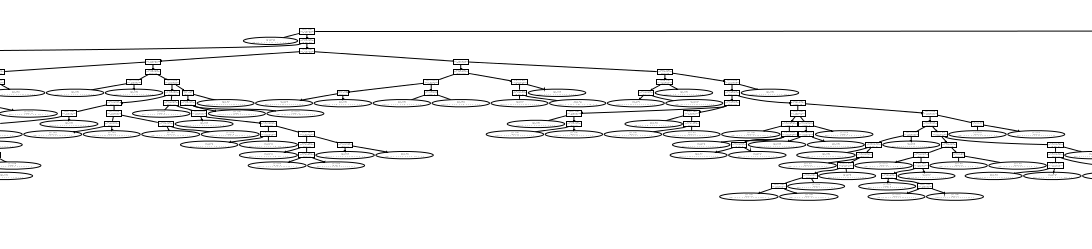
\includegraphics[scale=.25]{decisiontree_quarter.png}}
   \caption{Partial Decision Tree}
\end{figure}
\end{frame}

\begin{frame}
\frametitle{Decision tree vs Hash databases}
Evaluate precision \& recall:
\begin{itemize}
\item 5-Fold Stratified Cross Validation
\item 80 \% Train set, 20 \% Validation set
\end{itemize}

\begin{table}
\begin{tabular}{| c| c| c| c|}
\hline
Algorithm & Recall & Precision & F2-score\\
\hline
Hash & 1 & 2 & 3\\
Decision tree & 1 & 2 &3 \\
\hline
\end{tabular}
\end{table}
\end{frame}

\begin{frame}

\end{frame}

\begin{frame}
\end{frame}

\begin{frame}
\end{frame}

\begin{frame}

\end{frame}

\begin{frame}

\end{frame}


\section{Conclusion}
\begin{frame}
\frametitle{Conclusions}
\begin{itemize}
\item Parameters can be reduced to less than 
\item Decision tree has a better recall
\item Decision tree classifier has a better recall than 
\end{itemize}
~\\Future work:
\begin{itemize}
\item Compare to other learning algorithms
\item Extend feature set
\end{itemize}
\end{frame}

\section[Questions]{Questions}
\begin{frame}
~ \\~ \\~ \\
\begin{center}\Huge Questions? \end{center} 
\end{frame}

\begin{frame}[allowframebreaks]
        \frametitle{References}
        \bibliographystyle{unsrt}
        \bibliography{../report/scriptie_literatuur.bib}
\end{frame}


\end{document}